\documentclass[10pt]{article}

\usepackage[margin=0.6in]{geometry}
\usepackage{graphicx}
\usepackage{booktabs}
\usepackage[hidelinks]{hyperref}

\setlength{\parindent}{0pt}
\setlength{\parskip}{0.25em}

\begin{document}
\small

\begin{center}
{\Large \textbf{BRISC2025 Segmentation Inference Report}}\\
26 May 2026
\end{center}

\textbf{Goal.} This report summarizes the currently trained BRISC2025 stages, with focus on the single-kernel radial learning results and updated inference visuals.

\textbf{Method Overview.} The workflow includes: (1) selected-kernel classification from a broad filter bank, (2) a combined-kernel baseline, and (3) radial single-kernel optimization (seed, learned, and monotone-constrained variants).

\textbf{Structured and Combined Stages.}

\begin{center}
\begin{tabular}{lrrrr}
\toprule
\textbf{Model Stage} & \textbf{Val Acc} & \textbf{Val AUC} & \textbf{Test Acc} & \textbf{Test AUC} \\
\midrule
Selected-kernel classifier & 0.7398 & 0.8366 & 0.7715 & 0.8321 \\
Combined-kernel baseline & 0.6764 & 0.6994 & 0.6225 & 0.7013 \\
\bottomrule
\end{tabular}
\end{center}

\textbf{Single-Kernel Radial Stages.} The values below use the validation-tuned threshold.

\begin{center}
\begin{tabular}{lrrrr}
\toprule
\textbf{Radial Stage} & \textbf{Val Acc} & \textbf{Val AUC} & \textbf{Test Acc} & \textbf{Test AUC} \\
\midrule
Seed single-kernel radial & 0.7285 & 0.7012 & 0.6405 & 0.6961 \\
Learned single-kernel radial & 0.7536 & 0.7563 & 0.6740 & 0.7303 \\
Monotone-constrained radial & 0.6953 & 0.6801 & 0.6962 & 0.6268 \\
\bottomrule
\end{tabular}
\end{center}

The learned single-kernel stage improves over the seed radial baseline in both validation and test AUC, while the monotone-constrained version gives a more constrained shape and slightly different accuracy tradeoff.

% \textbf{Rotation-Invariant Kernel Figure.}\\
% 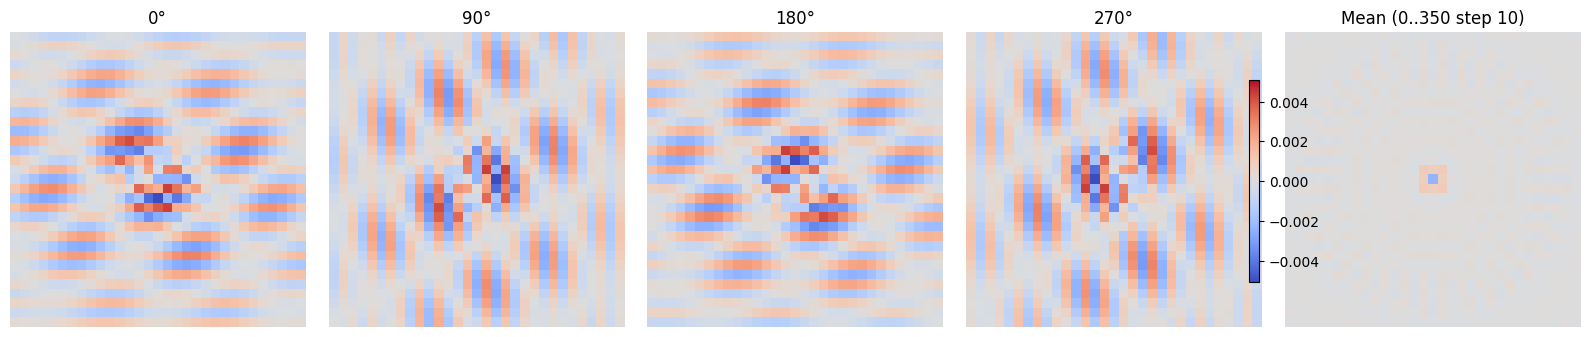
\includegraphics[width=0.92\textwidth]{figures/brisc2025_rotation_invariant_panel.png}

\textbf{Single-Kernel Trained Figure.}\\
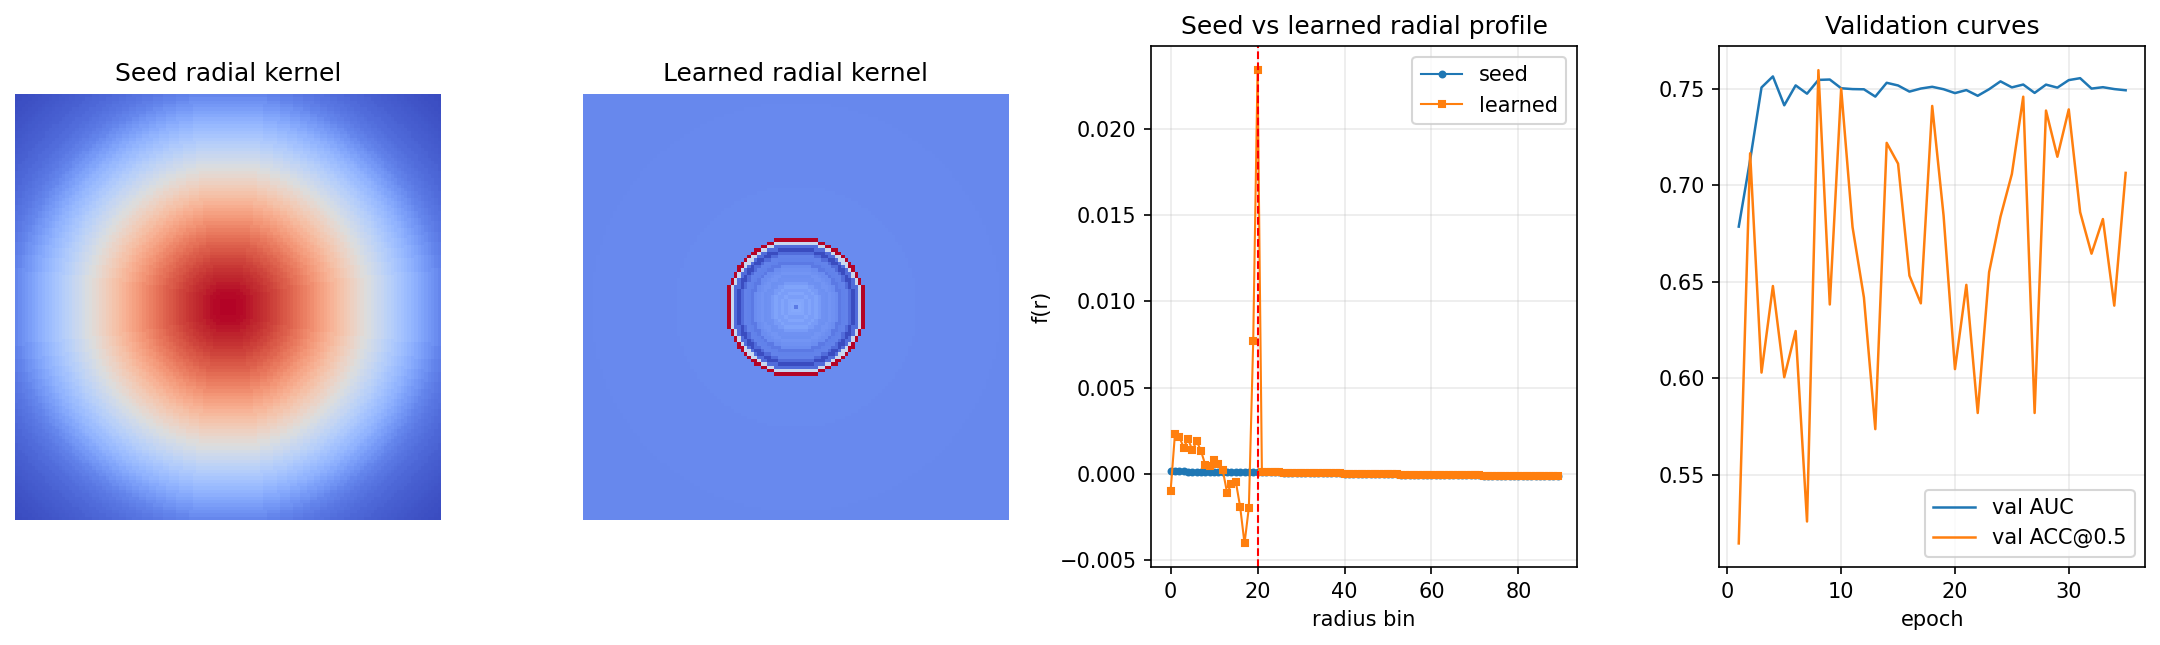
\includegraphics[width=0.92\textwidth]{figures/brisc2025_single_kernel_trained_summary.png}

% \textbf{Radial Kernel Shape.}\\
% 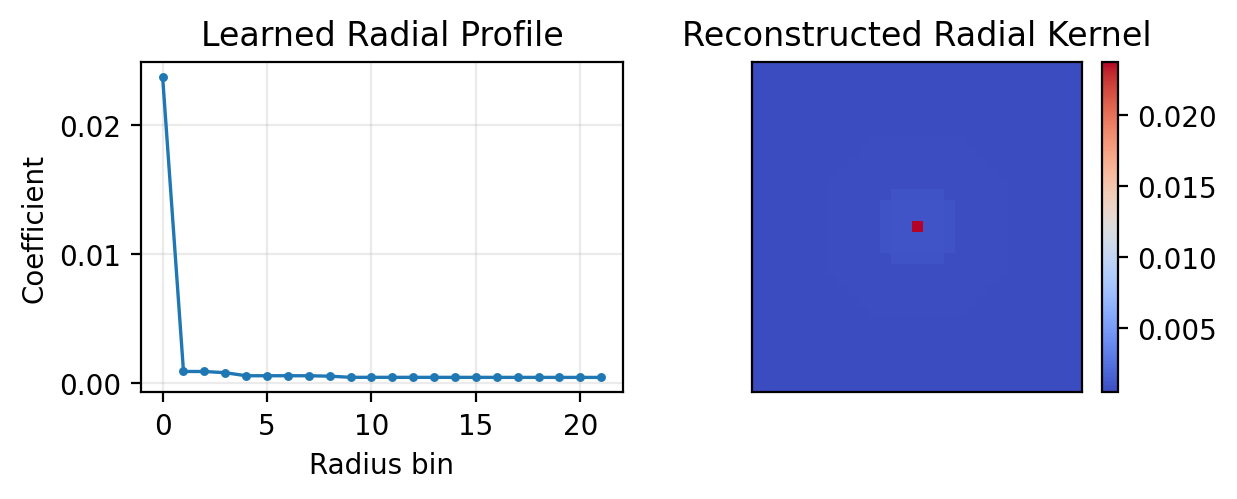
\includegraphics[width=0.72\textwidth]{figures/brisc2025_radial_kernel_summary.png}

\textbf{Structured-Kernel Heatmaps (Rows).}\\
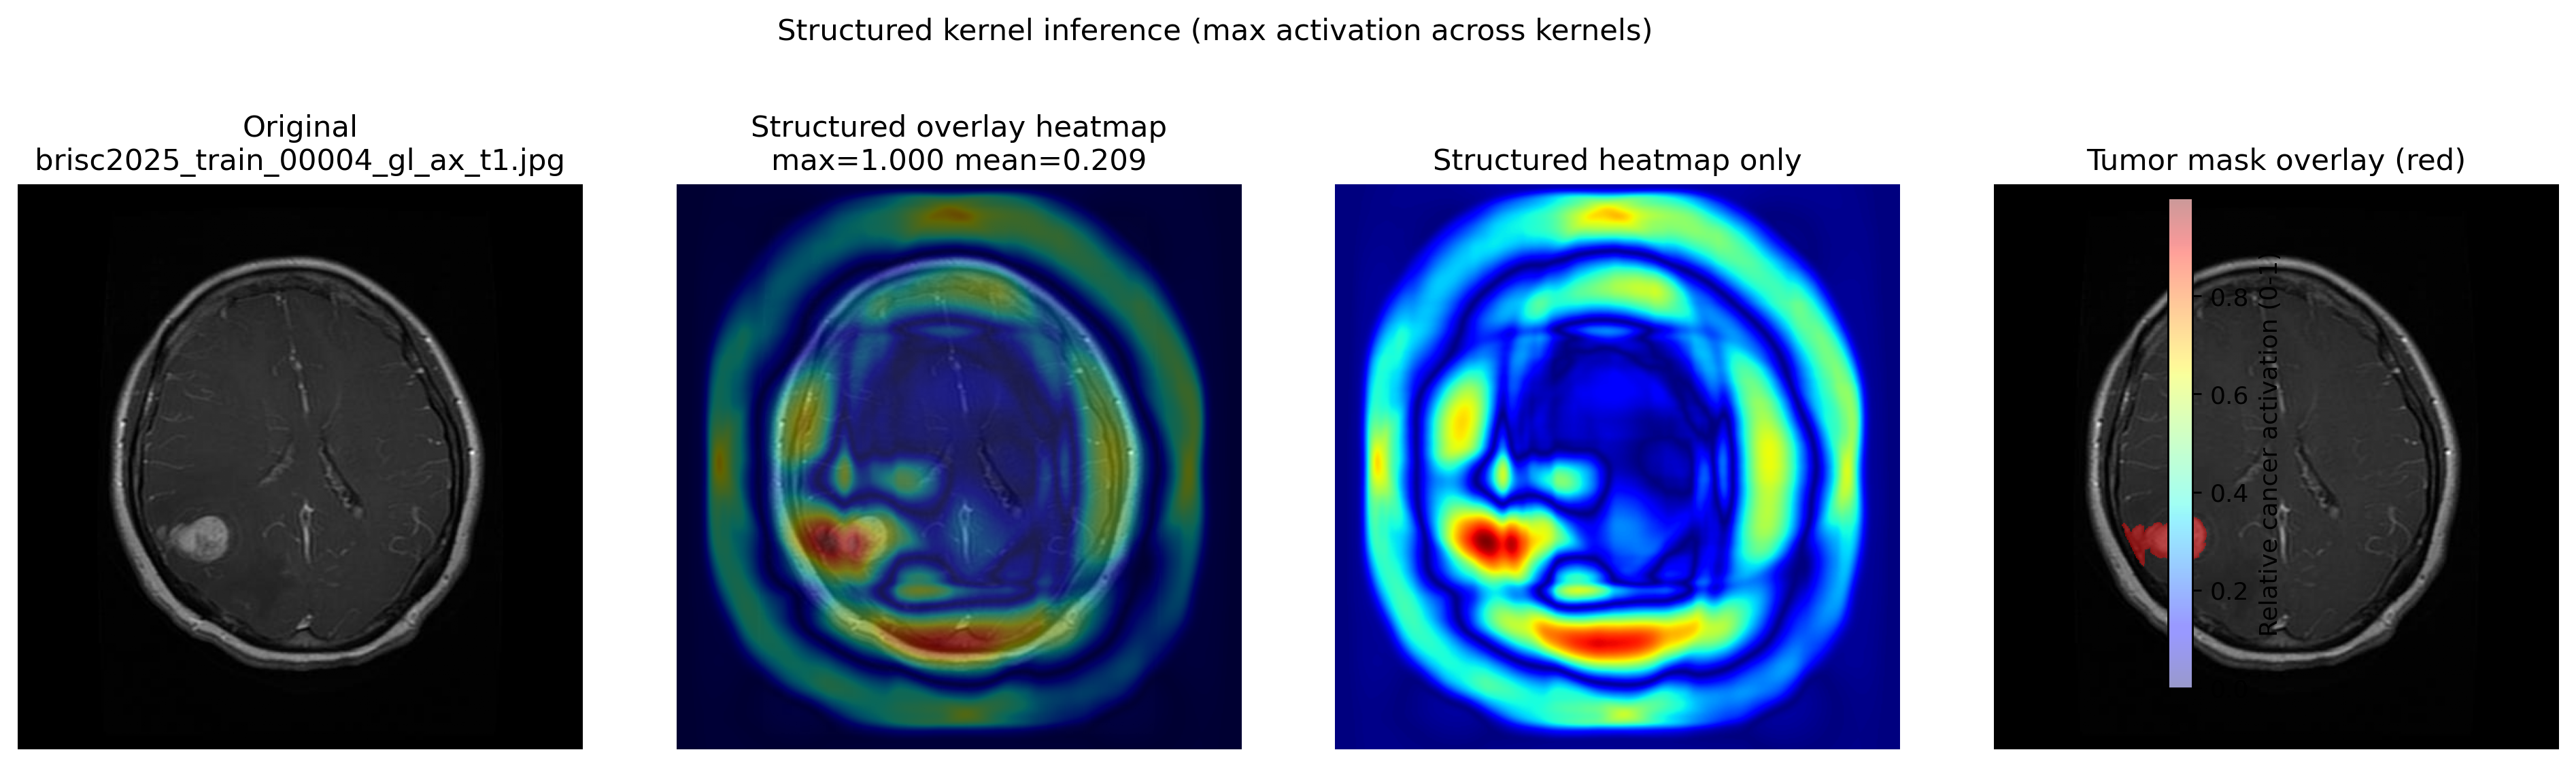
\includegraphics[width=0.82\textwidth]{../results/exp_brisc2025_mmr_nperFamily500_nComposition1250/brisc2025_train_00004_gl_ax_t1_structured_kernel_heatmap.png}\\
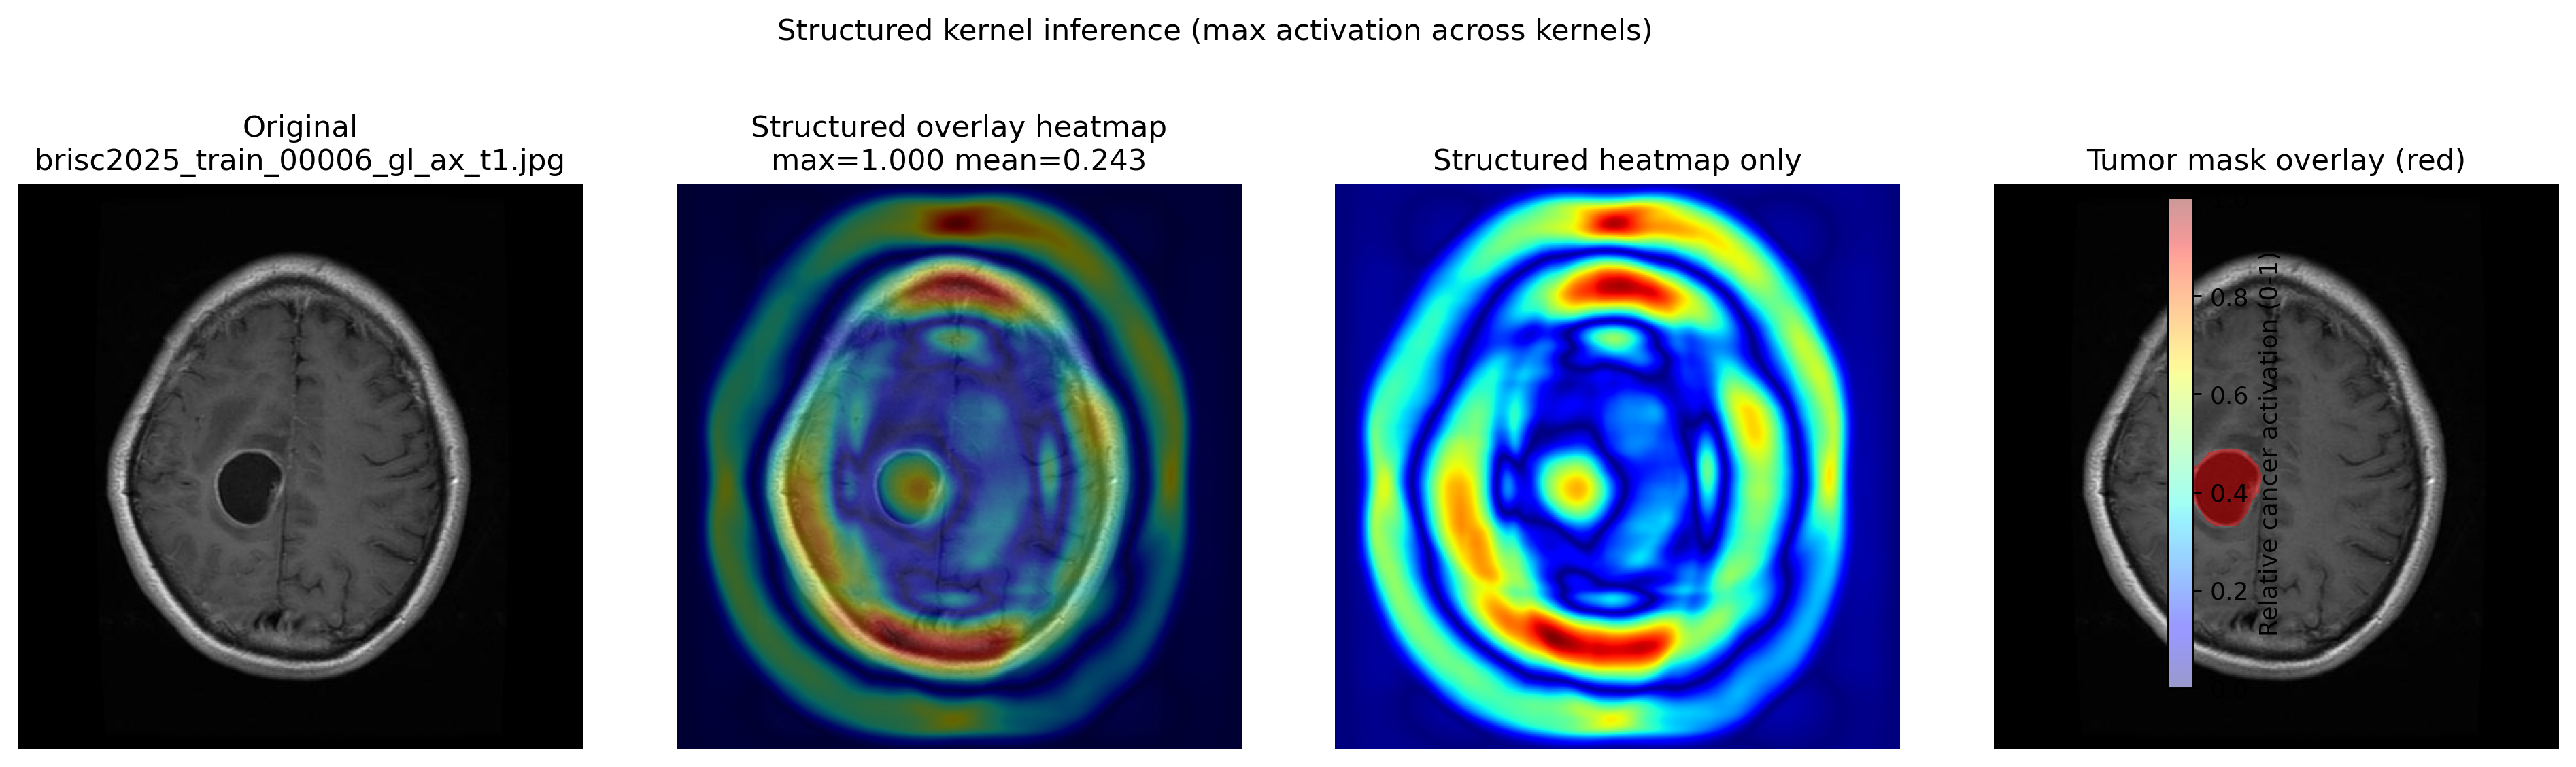
\includegraphics[width=0.82\textwidth]{../results/exp_brisc2025_mmr_nperFamily500_nComposition1250/brisc2025_train_00006_gl_ax_t1_structured_kernel_heatmap.png}\\
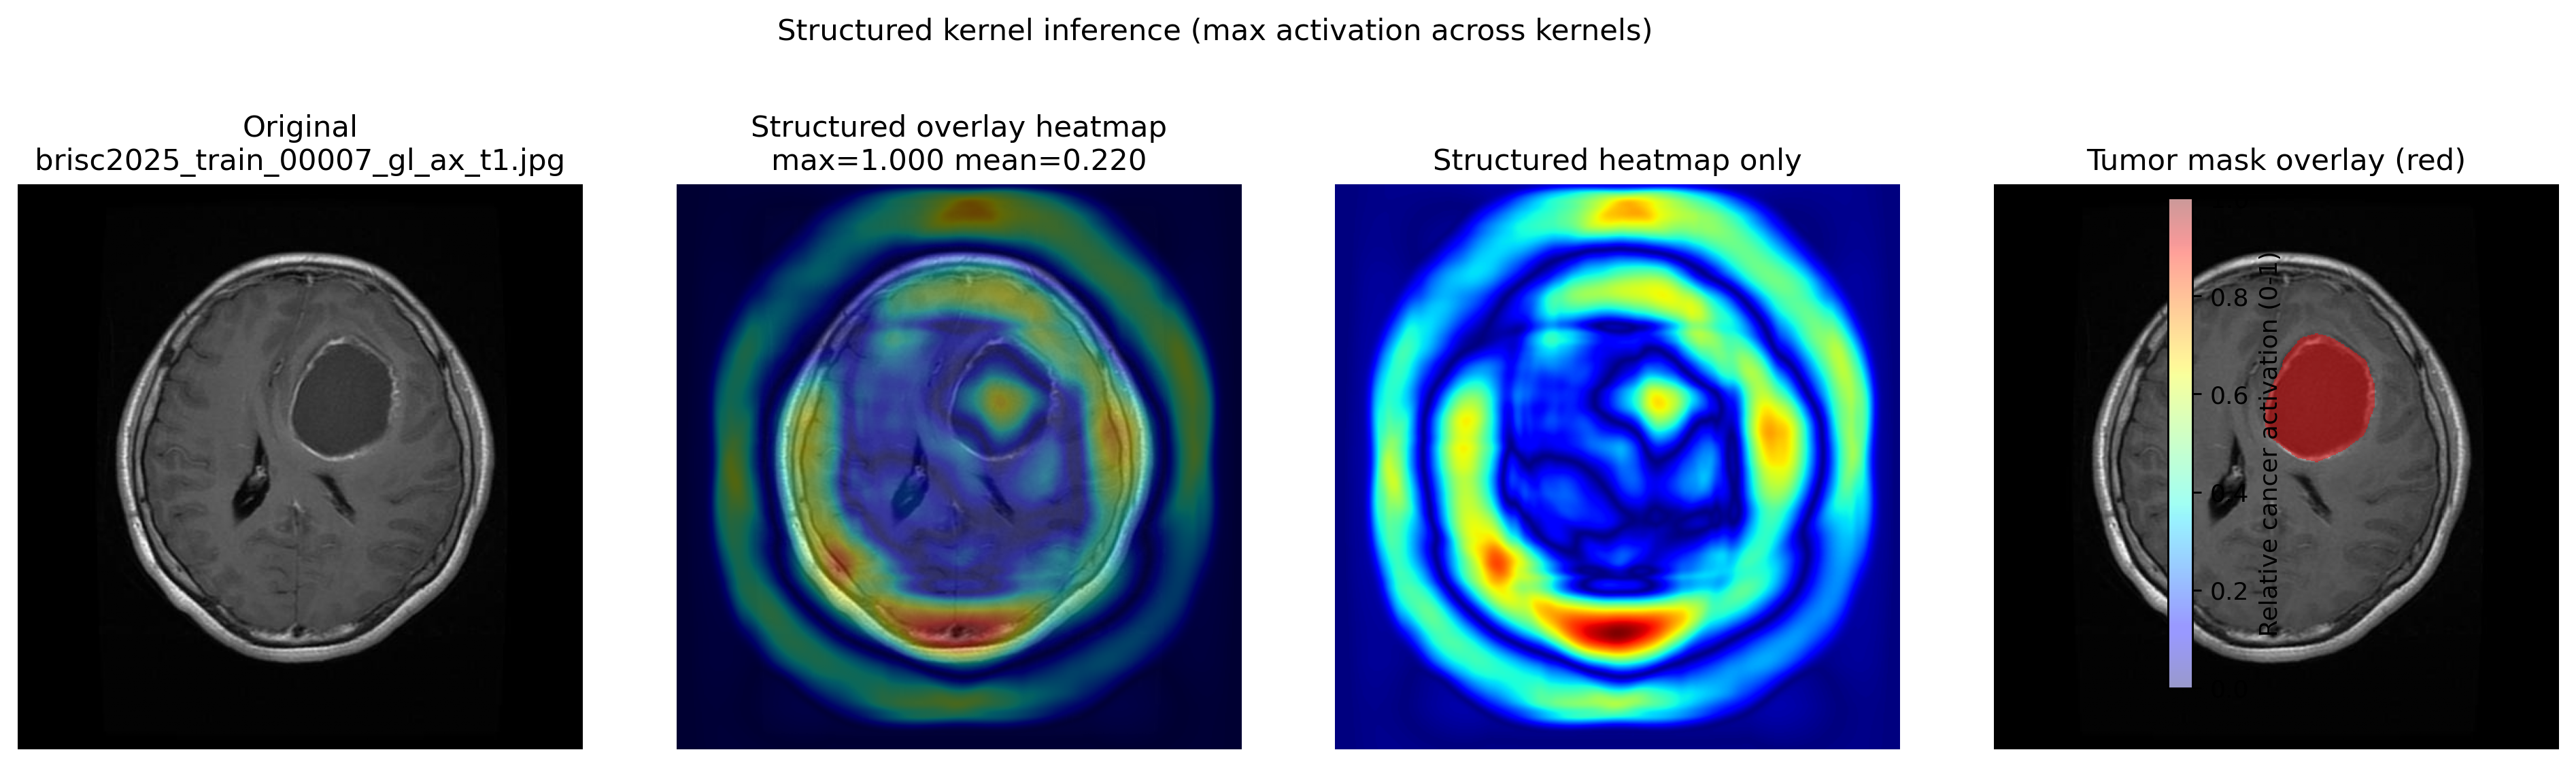
\includegraphics[width=0.82\textwidth]{../results/exp_brisc2025_mmr_nperFamily500_nComposition1250/brisc2025_train_00007_gl_ax_t1_structured_kernel_heatmap.png}\\
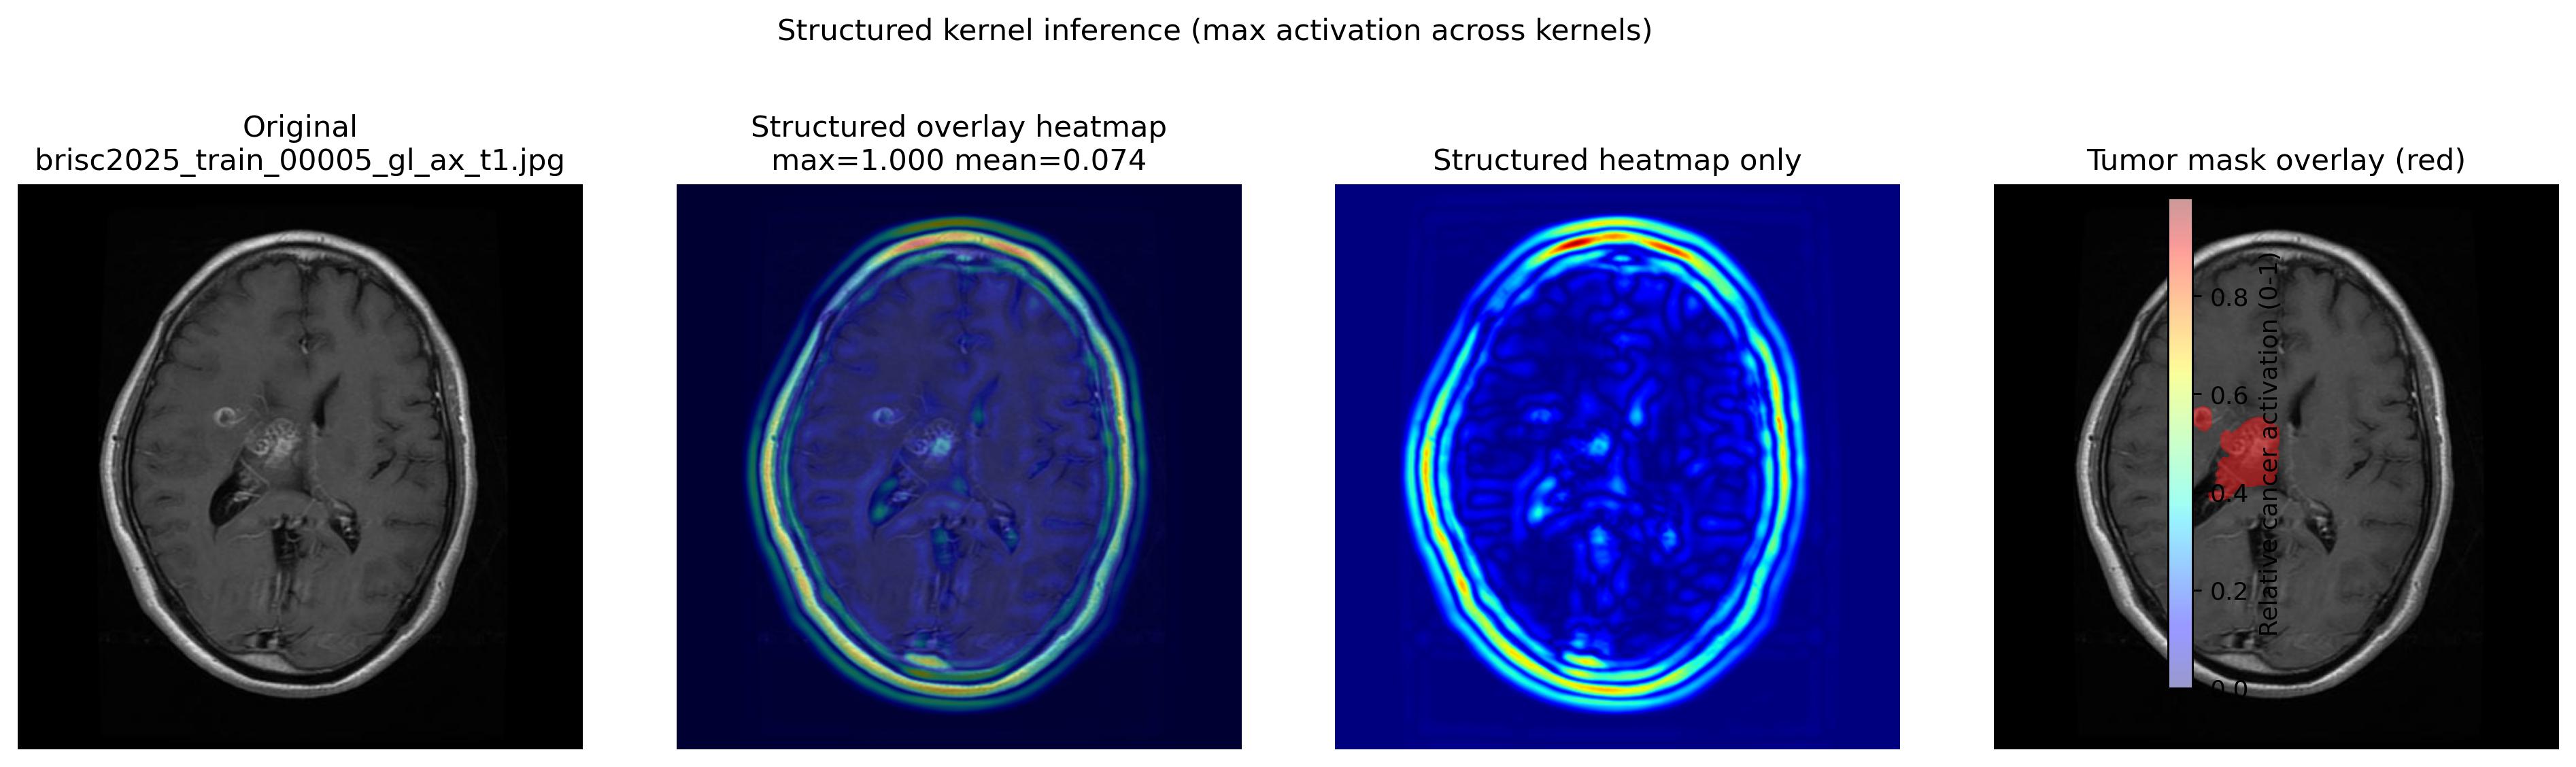
\includegraphics[width=0.82\textwidth]{../results/exp_brisc2025_mmr_nperFamily500_nComposition1250/brisc2025_train_00005_gl_ax_t1_structured_kernel_heatmap.png}

\textbf{Learned Radial Heatmaps (Rows).}\\
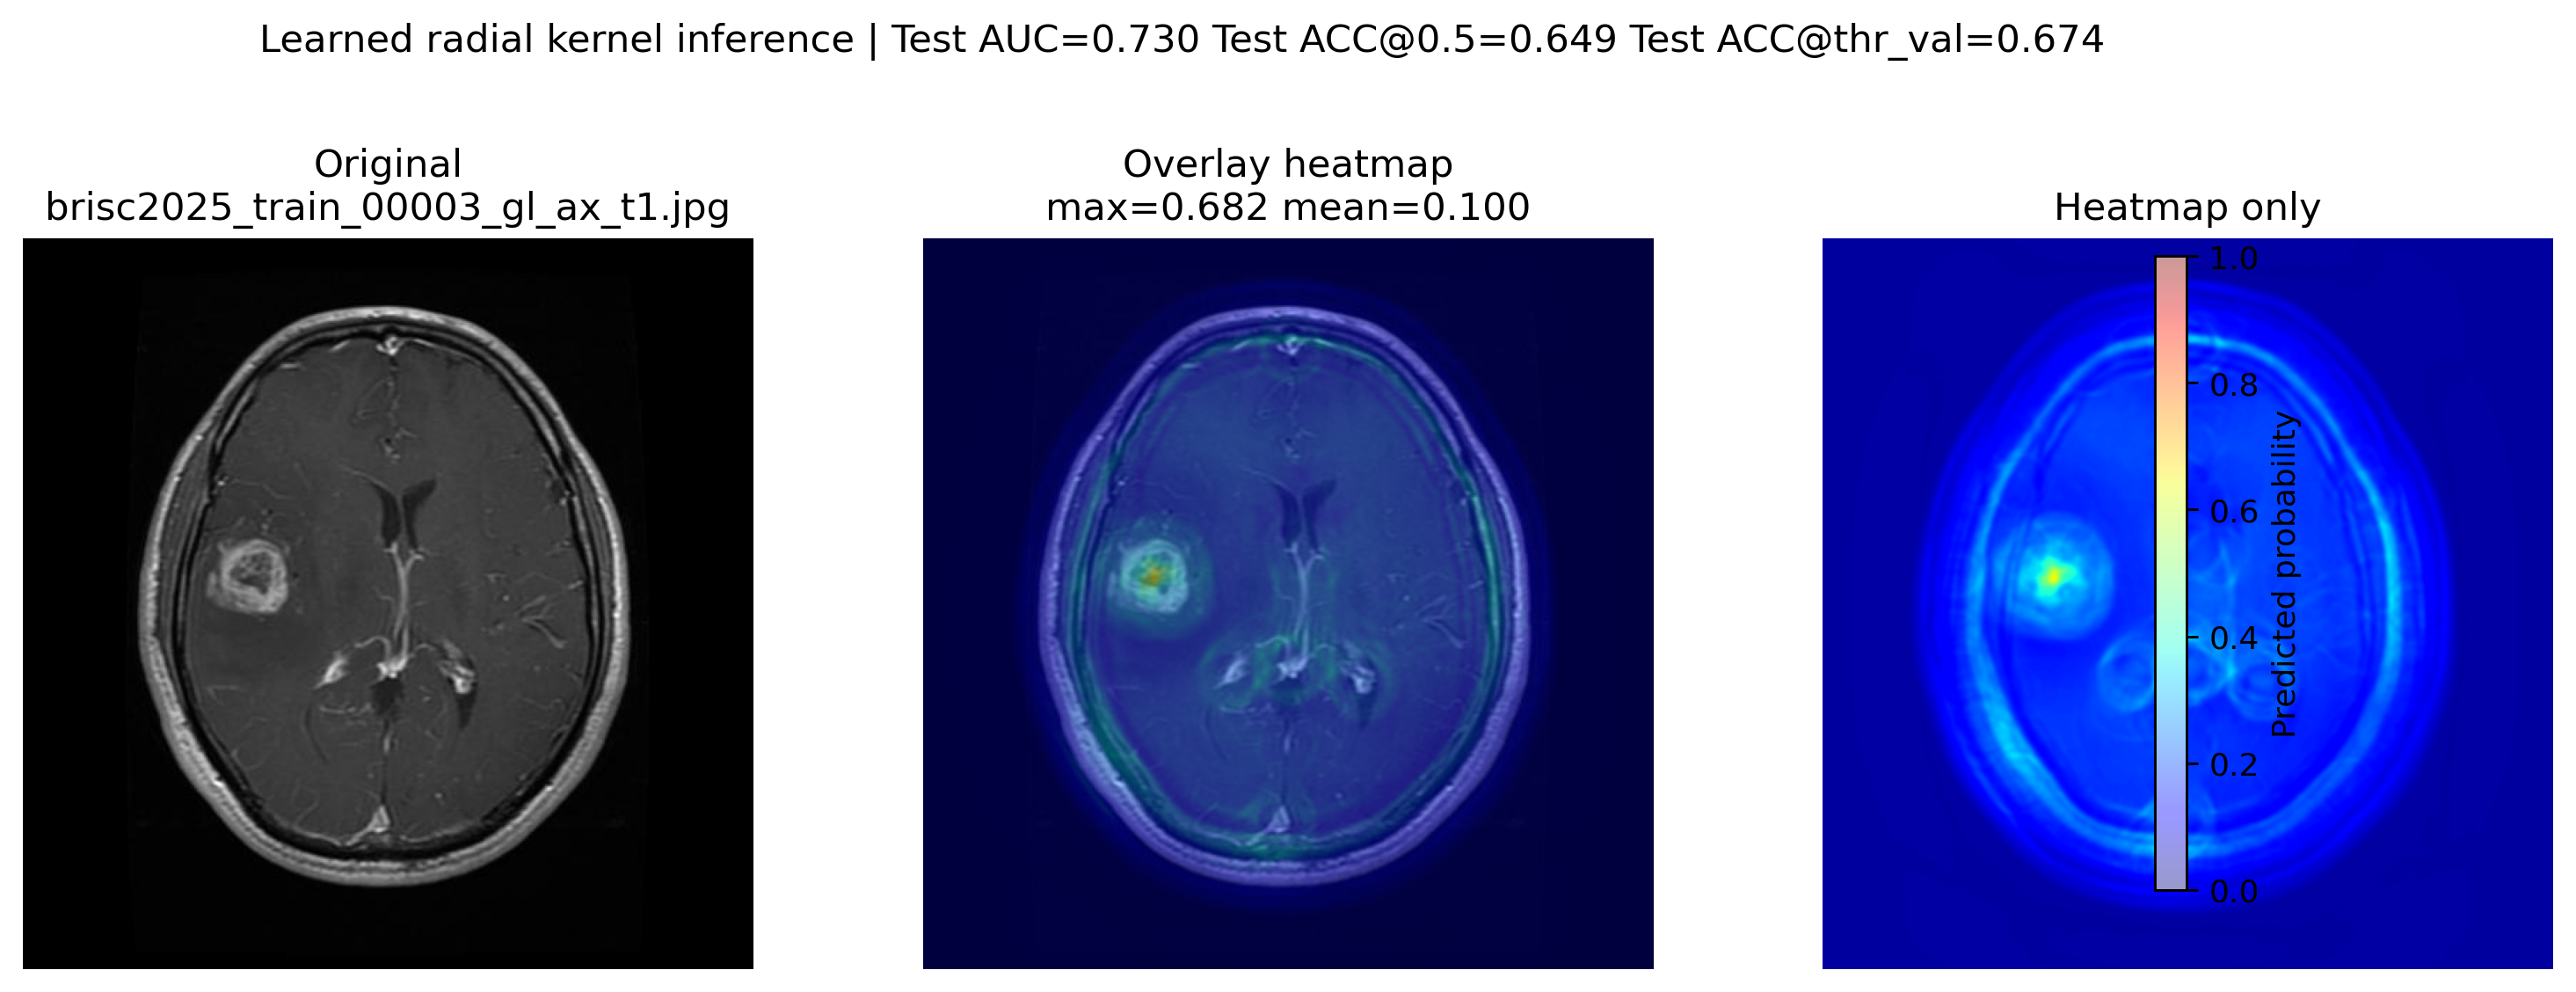
\includegraphics[width=0.82\textwidth]{../results/exp_brisc2025_mmr_nperFamily500_nComposition1250/radial_single_kernel_r20/brisc2025_train_00003_gl_ax_t1_learned_radial_heatmap.png}\\
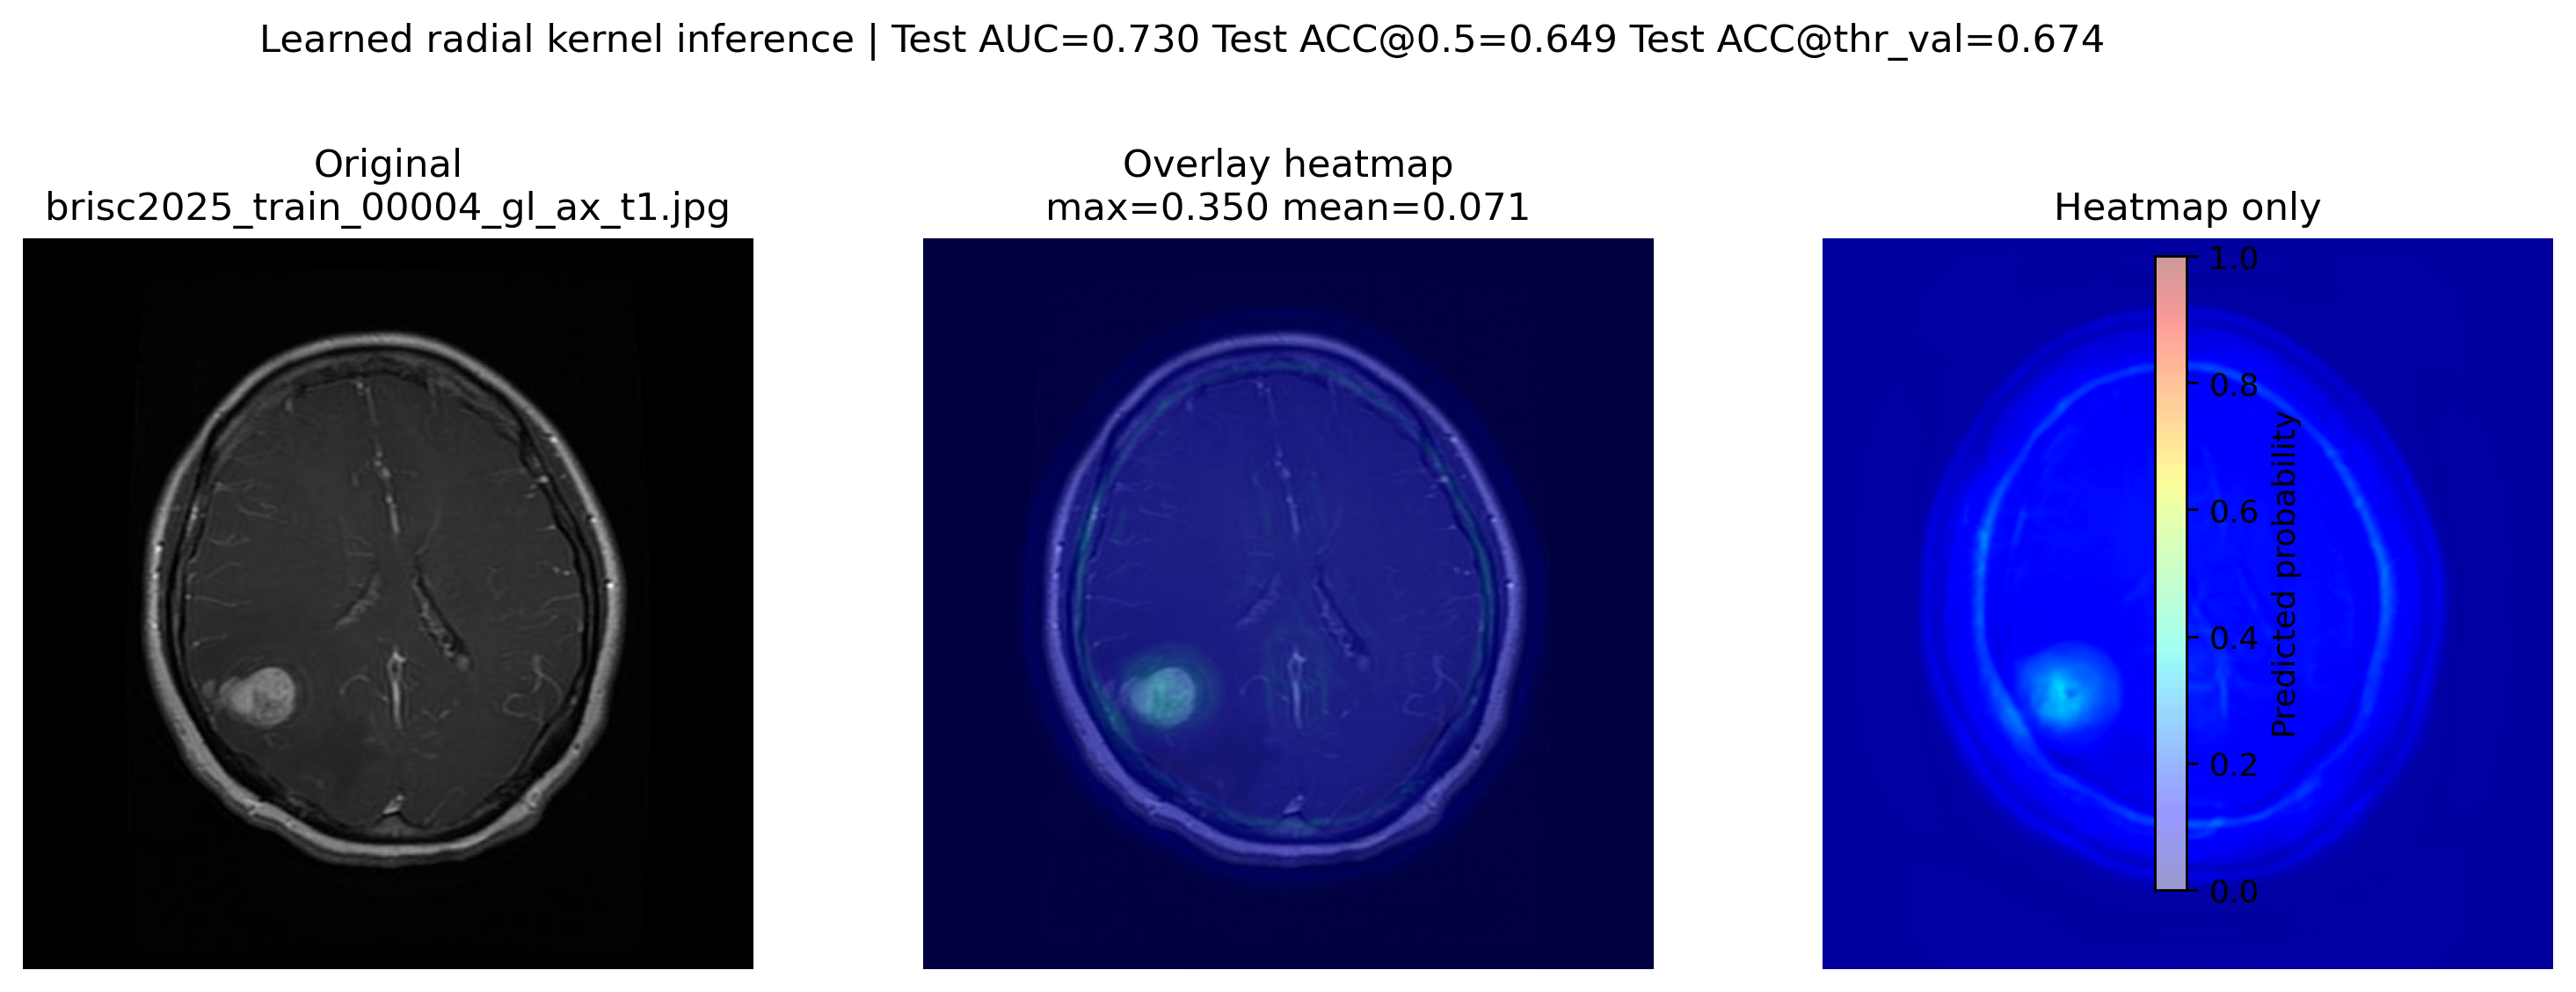
\includegraphics[width=0.82\textwidth]{../results/exp_brisc2025_mmr_nperFamily500_nComposition1250/radial_single_kernel_r20/brisc2025_train_00004_gl_ax_t1_learned_radial_heatmap.png}\\
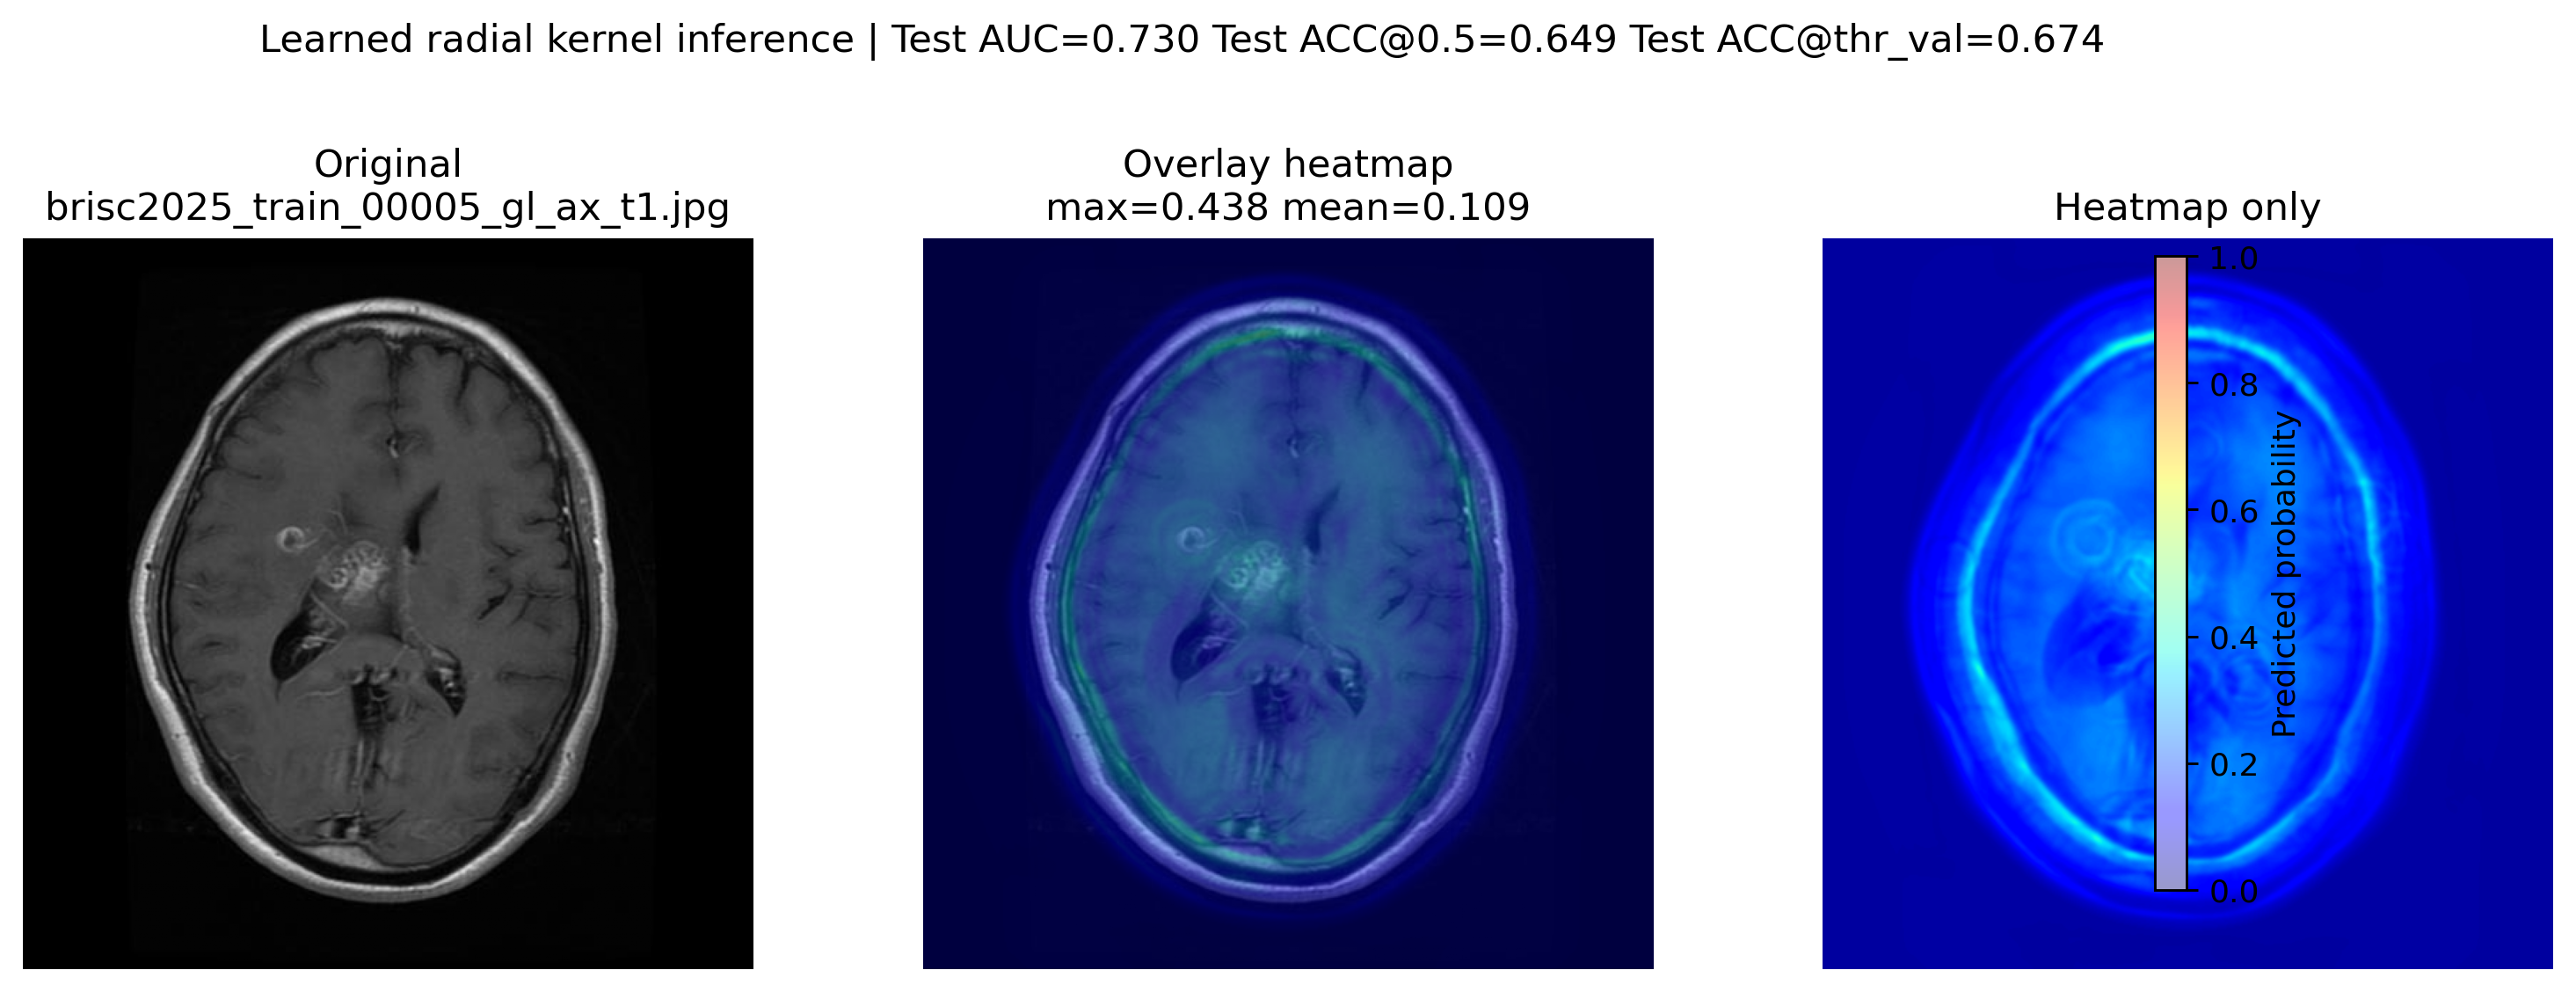
\includegraphics[width=0.82\textwidth]{../results/exp_brisc2025_mmr_nperFamily500_nComposition1250/radial_single_kernel_r20/brisc2025_train_00005_gl_ax_t1_learned_radial_heatmap.png}

\textbf{Conclusion.} The selected-kernel model remains strongest for final predictive quality, and the updated single-kernel radial training adds an interpretable local-response view with clear learned heatmaps across multiple BRISC2025 cases.

\end{document}
